% \documentclass[10pt,onecolumn]{article}
\documentclass[a4paper]{article}

\usepackage{amsmath, amsthm, amssymb,lscape, natbib,epstopdf,
	cases, bbm, indentfirst}
\usepackage{amsfonts}
\usepackage{graphicx}
\usepackage{epstopdf}
\usepackage{colortbl}
\usepackage[hang,small,bf]{caption}
\usepackage{setspace}
\usepackage{amsmath}
\usepackage[nohead]{geometry}
\usepackage[bottom]{footmisc}
\usepackage{endnotes}
\usepackage{rotating}
\usepackage{xr}
\usepackage{xr-hyper}
\usepackage[backref = section]{hyperref}
\usepackage[section]{placeins}
\allowdisplaybreaks
\usepackage{pdflscape}
\usepackage{float}

\usepackage{amsfonts}
\usepackage{graphicx}
\usepackage{epstopdf}
\usepackage{colortbl}
\usepackage{setspace}
\usepackage{amsmath}
\usepackage[nohead]{geometry}
\usepackage[bottom]{footmisc}
\usepackage{endnotes}
\usepackage{rotating}
\usepackage{xr}
\usepackage{xr-hyper}
\usepackage[backref = section]{hyperref}
\usepackage[section]{placeins}
\usepackage{amsmath}
\usepackage{caption}
\usepackage{subcaption}
\usepackage{pstricks}

\definecolor{citec}{rgb}{0,0,.5}
\definecolor{linkc}{rgb}{0,0,.6}
\definecolor{bcolor}{rgb}{1,1,1}

\hypersetup{
	colorlinks = true,
	urlcolor=linkc,
	linkcolor=linkc,
	citecolor = citec,
	filecolor = linkc,
	pdfauthor={Pat Moran}}

\usepackage{pstricks}
\usepackage{pstcol}

\onehalfspacing

%\input{tcilatex}
\geometry{left=1in,right=1.25in,top=1in,bottom=1in}
\interfootnotelinepenalty=10000

\begin{document}	
	%-------------------------------------------------
	\title{Household expenditure in retirement}
	\date{}
	\maketitle

%-------------------------------------------------
\section{Income by Duration of Retirement}

\begin{figure}[h]
	\caption{Income Around Retirement}
	\centering
	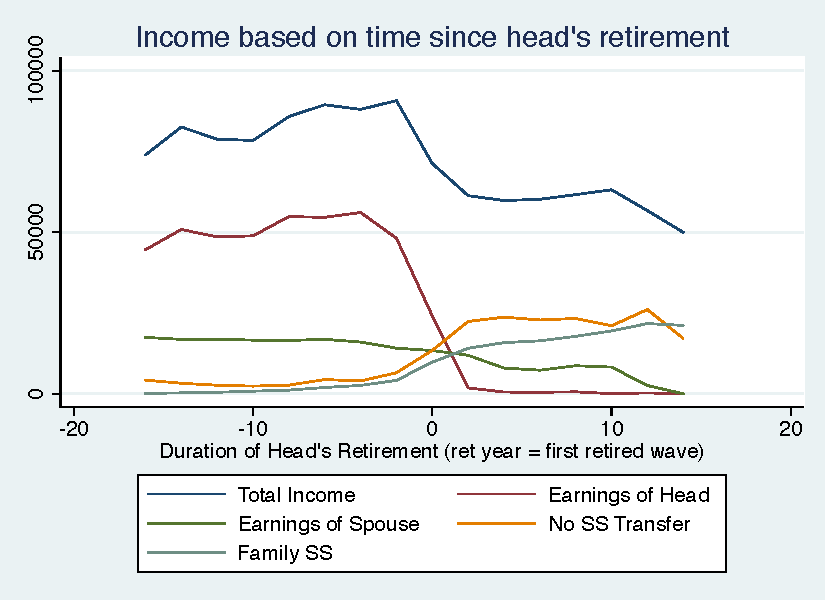
\includegraphics[width=1.0\textwidth]{../IncomeAroundRetirement/Income_with_spouse_definition_1.pdf}
\end{figure}

Here we use the full sample - we do not select HHs based on spouse behavior. Though of course the results vary greatly if we look at households where the spouse does not work, always works, etc. 
%inc_fam - "Total Income". "Inc Head" - "Earnings of Head" inc_spouse "Earnings of Spounds" inc_transfer "No SS Transfer", inc_ss_fam "Family SS"

\clearpage

\section{Expenditure Breakdown by Duration of Retirement}

\begin{figure}[h]
	\caption{Expenditure Breakdown for the Bottom Tertile - for categories before 2005}
	\centering
	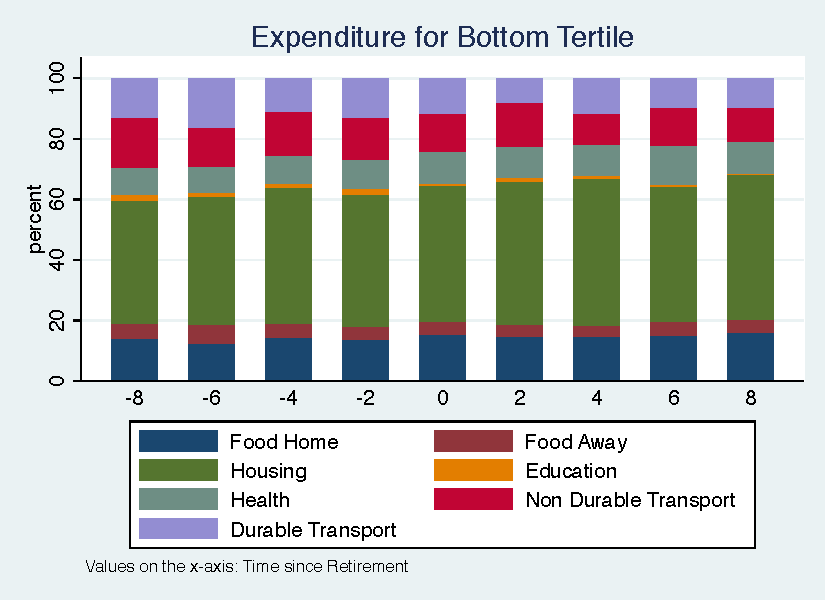
\includegraphics[width=0.9\textwidth]{../ConsumptionPostRetirement/Tertile_Bar/tertile1.pdf}
\end{figure}

%\begin{figure}[h]
%	\caption{For categories before 2005}
%	\centering
%	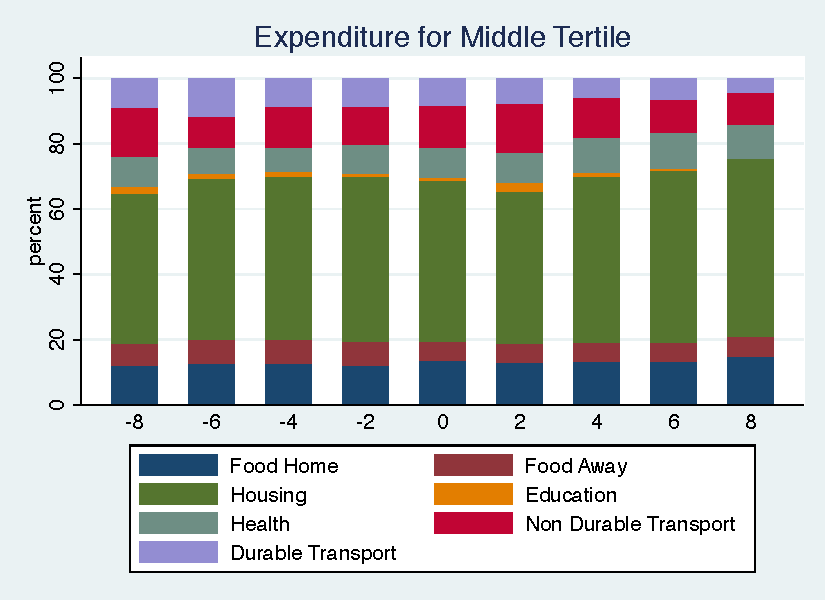
\includegraphics[width=0.8\textwidth]{../ConsumptionPostRetirement/Tertile_Bar/tertile2.pdf}
%\end{figure}

\begin{figure}[H]
	\caption{Expenditure Breakdown for the Top Tertile - for categories before 2005}
	\centering
	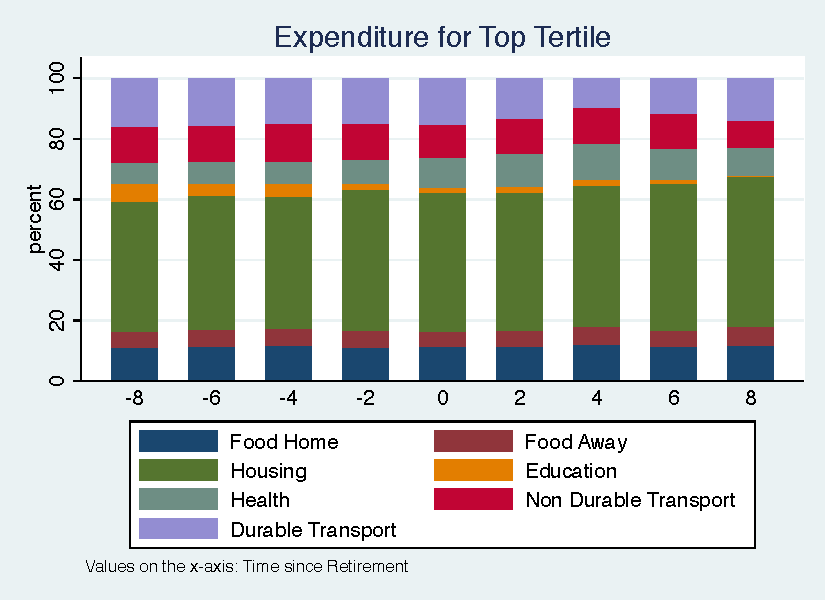
\includegraphics[width=0.9\textwidth]{../ConsumptionPostRetirement/Tertile_Bar/tertile3.pdf}
\end{figure}


\clearpage


%-------------------------------------------------
\section{Total Nondurable expenditure (unsmoothed)}

\begin{figure}[h]
	\caption{Full Sample - Total Nondurable expenditure}
	\centering
	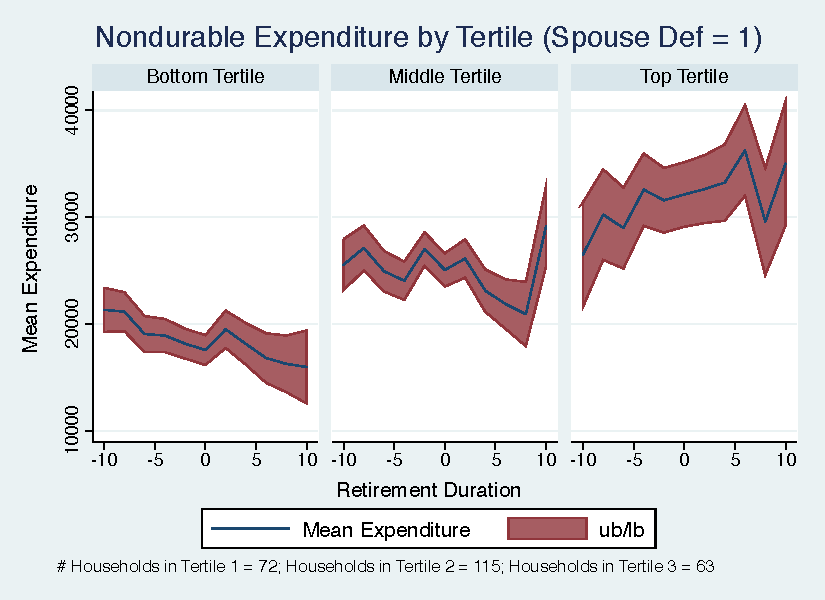
\includegraphics[width=0.9\textwidth]{../ConsumptionPostRetirement_by_SpouseDef/UnSmoothed/spouse_def_1.pdf}
\end{figure}



\begin{figure}[H]
	\caption{Spouse Never Works- Total Nondurable expenditure}
	\centering
	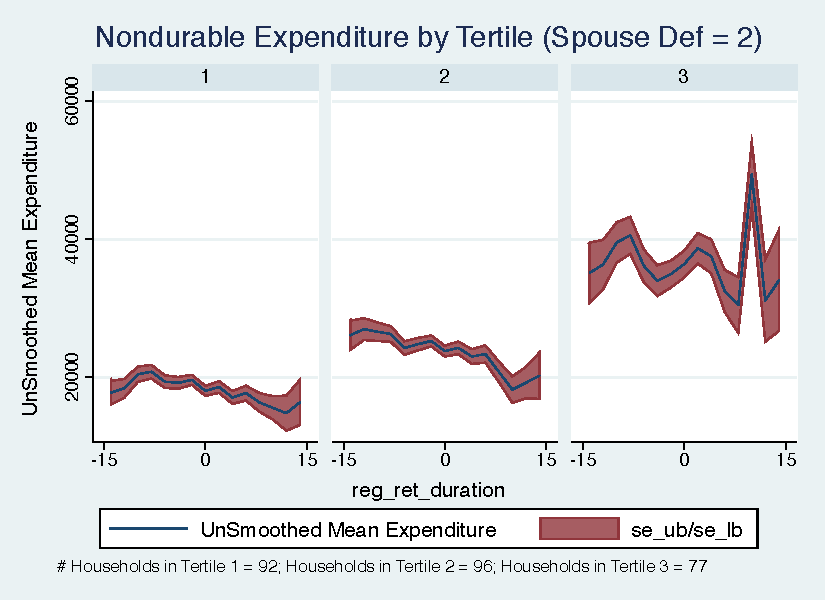
\includegraphics[width=0.9\textwidth]{../ConsumptionPostRetirement_by_SpouseDef/UnSmoothed/spouse_def_2.pdf}
\end{figure}


\begin{figure}[H]
	\caption{Spouse Always Works- Total Nondurable expenditure}
	\centering
	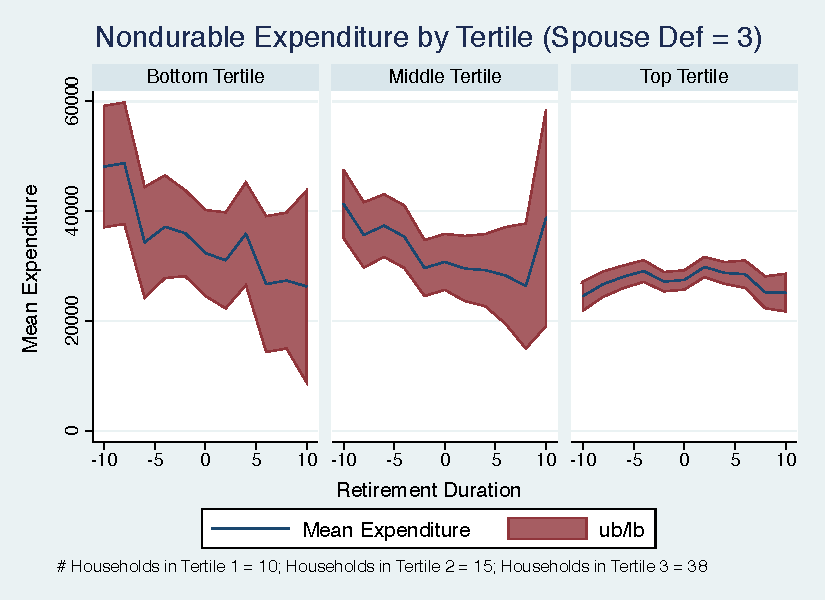
\includegraphics[width=0.9\textwidth]{../ConsumptionPostRetirement_by_SpouseDef/UnSmoothed/spouse_def_3.pdf}
\end{figure}

Full sample: Expenditure falls slightly for all three tertiles

Spouse never works: Expenditure falls slightly for all three tertiles

Spouse always works: Expenditure rises slightly for the rich

\clearpage





%-------------------------------------------------
\section{Expenditure based on tertiles (smoothed)} 
\begin{figure}[h]
	\caption{Expenditure based on tertile}
	\begin{subfigure}{1.0\textwidth}
		\centering
		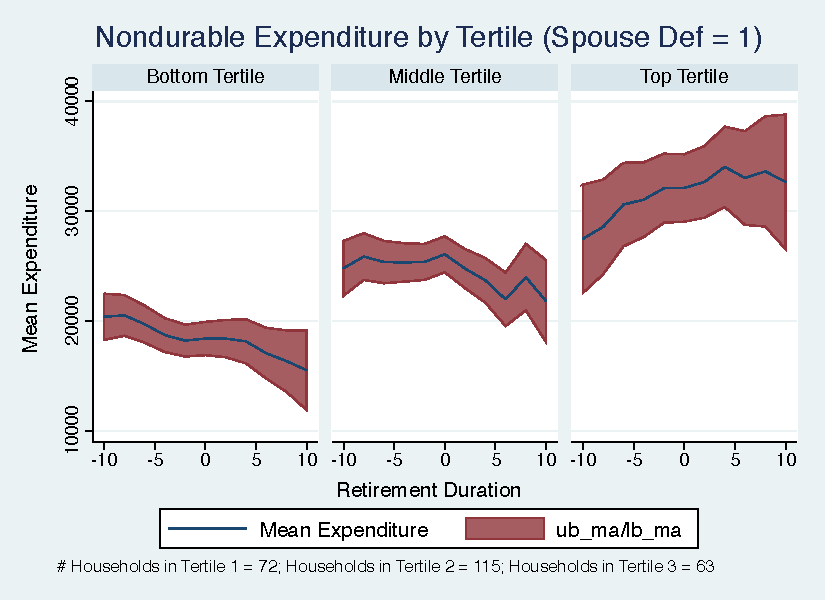
\includegraphics[width=0.8\linewidth]{../ConsumptionPostRetirement_by_SpouseDef/Smoothed/spouse_def_1.pdf}
		\caption{Nondurable expenditure}
	\end{subfigure}
	\vspace{1cm}
	
	\begin{subfigure}{0.5\textwidth}
		\centering
		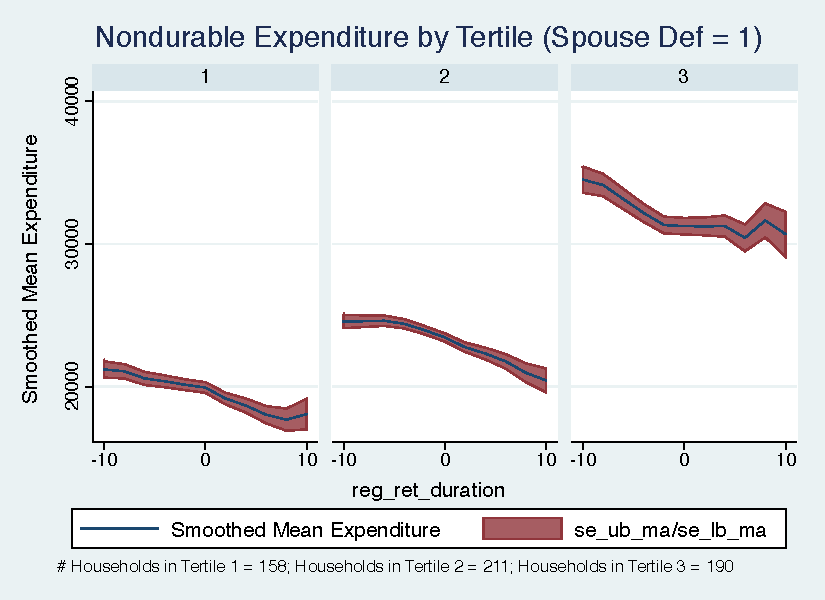
\includegraphics[width=0.9\linewidth]{../ConsumptionPostRetirement_by_SpouseDef/Smoothed_xhealth/spouse_def_1.pdf}
		\caption{Nondurables w/o health exp}
		\label{fig:chapter001_dist_001}
	\end{subfigure}
	\hspace{1cm}
	\begin{subfigure}{0.5\textwidth}
		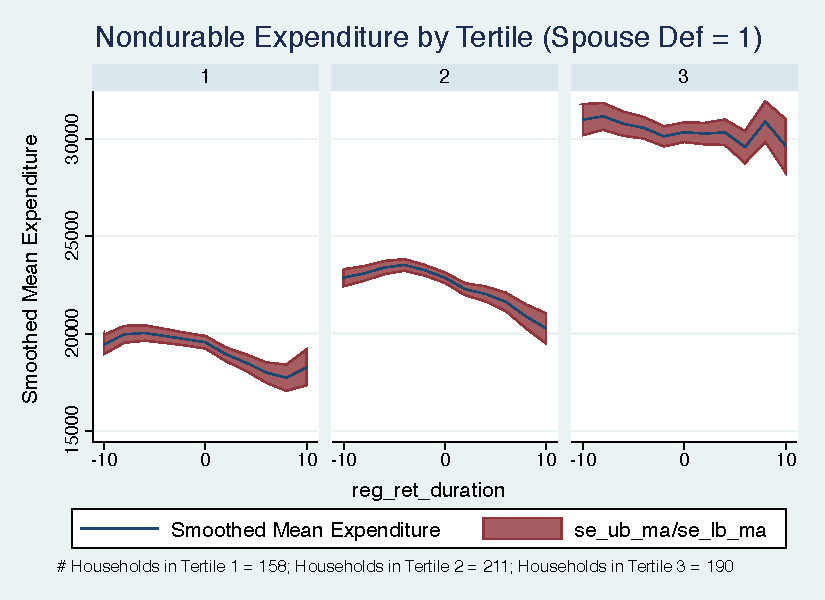
\includegraphics[width=0.9\linewidth]{../ConsumptionPostRetirement_by_SpouseDef/Smoothed_xhealth_educ/spouse_def_1.pdf}
		\caption{Nondurables w/o health and educ exp}
		\label{fig:chapter001_reward_001}
	\end{subfigure}
\end{figure}

Here we use the full sample - we do not select HHs based on spouse behavior.

Expenditure is roughly flat for the top tertile, once you take away education expenditure.

If spouse always works it's similar, if spouse different it looks similar, if spouse never works looks different
\clearpage


%-------------------------------------------------
\begin{landscape}
\section{Expenditure Regressions}

Here we use the full sample - we do not select households based upon spouse behavior

\subsection{Regression table with nondurables expenditure}
\begin{tabular}{lcccccccccc} \hline
 & (1) & (2) & (3) & (4) & (5) & (6) & (7) & (8) & (9) & (10) \\
VARIABLES & OLS & test 2 & test 3 & test 4 & test 5 & test 6 & test 7 & test 8 & test 9 & test 10 \\ \hline
 &  &  &  &  &  &  &  &  &  &  \\
1.retired & 8,504*** & 2,291*** & 1,276 & 991.5 & 1,364 & 1,486 & 2,291*** & -1,371 & -1,038 & 185.7 \\
 & (1,121) & (875.7) & (868.9) & (861.2) & (854.1) & (1,422) & (869.7) & (1,308) & (1,286) & (1,344) \\
 &  &  &  &  &  &  &  &  &  &  \\
Observations & 69,862 & 69,862 & 69,862 & 69,862 & 69,862 & 640 & 640 & 640 & 640 & 640 \\
R-squared & 0.001 & 0.000 & 0.040 & 0.057 & 0.073 & 0.002 & 0.012 & 0.116 & 0.154 & 0.191 \\
HH FE & No & Yes & Yes & Yes & Yes & No & Yes & Yes & Yes & Yes \\
Age Dummies & No & No & Yes & Yes & Yes & No & No & Yes & Yes & Yes \\
Dummy Children & No & No & No & Yes & Yes & No & No & No & Yes & Yes \\
Time & No & No & No & No & Yes & No & No & No & No & Yes \\
 Number of pid &  & 18,085 & 18,085 & 18,085 & 18,085 &  & 86 & 86 & 86 & 86 \\ \hline
\multicolumn{11}{c}{ Standard errors in parentheses} \\
\multicolumn{11}{c}{ *** p$<$0.01, ** p$<$0.05, * p$<$0.1} \\
\end{tabular}

\clearpage

\subsection{Regression table with nondurables expenditure w/o health expenditure} 
\begin{tabular}{lcccccccccc} \hline
 & (1) & (2) & (3) & (4) & (5) & (6) & (7) & (8) & (9) & (10) \\
VARIABLES & OLS & test 2 & test 3 & test 4 & test 5 & test 6 & test 7 & test 8 & test 9 & test 10 \\ \hline
 &  &  &  &  &  &  &  &  &  &  \\
2.tertile & 4,913*** & 900.3** & 52.98 & -89.01 & -152.7 & 4,257** & -5,729 & -11,352 & -11,005 & -10,348 \\
 & (182.9) & (363.4) & (358.2) & (353.4) & (350.1) & (1,869) & (9,399) & (9,575) & (9,397) & (9,258) \\
3.tertile & 14,455*** & 1,047** & -221.0 & -162.9 & 14.37 & 8,754*** & 2,351 & -10,782 & -11,571 & -6,813 \\
 & (198.2) & (426.4) & (421.3) & (415.6) & (411.7) & (1,989) & (11,102) & (11,649) & (11,411) & (11,276) \\
1.retired\#1b.tertile & 8,513*** & 267.5 & 617.2 & 41.83 & 42.72 & -570.9 & 267.5 & -2,327 & -2,543 & -581.4 \\
 & (1,985) & (1,597) & (1,598) & (1,576) & (1,561) & (2,736) & (1,669) & (2,018) & (1,983) & (2,012) \\
1.retired\#2.tertile & 8,991*** & -825.5 & -1,121 & -1,017 & -987.6 & 563.1 & -807.8 & -3,177* & -2,481 & -641.3 \\
 & (1,417) & (1,230) & (1,239) & (1,223) & (1,211) & (2,031) & (1,286) & (1,617) & (1,593) & (1,647) \\
1.retired\#3.tertile & 1,253 & 1,215 & 892.8 & 761.9 & 685.9 & -2,130 & 1,085 & -701.8 & -406.6 & 1,167 \\
 & (1,781) & (1,445) & (1,469) & (1,449) & (1,435) & (2,486) & (1,513) & (1,831) & (1,796) & (1,826) \\
 &  &  &  &  &  &  &  &  &  &  \\
Observations & 46,591 & 46,591 & 46,591 & 46,591 & 46,591 & 623 & 623 & 623 & 623 & 623 \\
R-squared & 0.128 & 0.000 & 0.041 & 0.067 & 0.085 & 0.039 & 0.006 & 0.090 & 0.133 & 0.176 \\
HH FE & No & Yes & Yes & Yes & Yes & No & Yes & Yes & Yes & Yes \\
Age Dummies & No & No & Yes & Yes & Yes & No & No & Yes & Yes & Yes \\
Dummy Children & No & No & No & Yes & Yes & No & No & No & Yes & Yes \\
Time & No & No & No & No & Yes & No & No & No & No & Yes \\
 Number of pid &  & 11,778 & 11,778 & 11,778 & 11,778 &  & 79 & 79 & 79 & 79 \\ \hline
\multicolumn{11}{c}{ Standard errors in parentheses} \\
\multicolumn{11}{c}{ *** p$<$0.01, ** p$<$0.05, * p$<$0.1} \\
\end{tabular}

\clearpage

\subsection{Regression table with nondurables expenditure without Health and Education Expenditure}
\begin{tabular}{lcccccccccc} \hline
 & (1) & (2) & (3) & (4) & (5) & (6) & (7) & (8) & (9) & (10) \\
VARIABLES & OLS & test 2 & test 3 & test 4 & test 5 & test 6 & test 7 & test 8 & test 9 & test 10 \\ \hline
 &  &  &  &  &  &  &  &  &  &  \\
1.retired & 4,649*** & -721.5*** & -1,210*** & -1,231*** & -1,163*** & -624.0 & -721.5** & -1,441*** & -1,421*** & -1,004** \\
 & (311.3) & (266.0) & (289.1) & (287.4) & (284.5) & (462.0) & (289.8) & (419.1) & (417.0) & (414.2) \\
 &  &  &  &  &  &  &  &  &  &  \\
Observations & 69,862 & 69,862 & 69,862 & 69,862 & 69,862 & 4,489 & 4,489 & 4,489 & 4,489 & 4,489 \\
R-squared & 0.003 & 0.000 & 0.028 & 0.040 & 0.060 & 0.000 & 0.002 & 0.124 & 0.134 & 0.169 \\
HH FE & No & Yes & Yes & Yes & Yes & No & Yes & Yes & Yes & Yes \\
Age Dummies & No & No & Yes & Yes & Yes & No & No & Yes & Yes & Yes \\
Dummy Children & No & No & No & Yes & Yes & No & No & No & Yes & Yes \\
Time & No & No & No & No & Yes & No & No & No & No & Yes \\
 Number of pid &  & 18,085 & 18,085 & 18,085 & 18,085 &  & 582 & 582 & 582 & 582 \\ \hline
\multicolumn{11}{c}{ Standard errors in parentheses} \\
\multicolumn{11}{c}{ *** p$<$0.01, ** p$<$0.05, * p$<$0.1} \\
\end{tabular}

\clearpage


\section{Expenditure Regressions: interact retirement with tertiles}

Here we use the full sample - we do not select households based upon spouse behavior
Note: smaller sample size is due to the approximately 20k HHs who do not have tertile defined (due to no social security observations)

\subsection{Regression table with nondurables expenditure}
\begin{tabular}{lcccccccccc} \hline
 & (1) & (2) & (3) & (4) & (5) & (6) & (7) & (8) & (9) & (10) \\
VARIABLES & OLS & test 2 & test 3 & test 4 & test 5 & test 6 & test 7 & test 8 & test 9 & test 10 \\ \hline
 &  &  &  &  &  &  &  &  &  &  \\
1.retired\#1b.tertile & 2,678*** & -2,190** & -2,222** & -2,103** & -2,305*** & -2,645* & -2,190** & -1,771 & -1,946* & -1,398 \\
 & (903.0) & (875.7) & (913.2) & (901.8) & (894.0) & (1,442) & (1,068) & (1,178) & (1,172) & (1,174) \\
1.retired\#2.tertile & 848.8 & -1,107 & -541.6 & -387.8 & -877.4 & -2,122 & -1,107 & 36.42 & -117.1 & 32.38 \\
 & (793.6) & (777.6) & (824.8) & (814.5) & (807.6) & (1,290) & (948.7) & (1,090) & (1,083) & (1,078) \\
1.retired\#3.tertile & 7,788*** & 898.8 & 1,025 & 1,232 & 907.2 & 5,541*** & 898.8 & 1,317 & 1,174 & 1,558 \\
 & (830.3) & (786.9) & (834.9) & (824.5) & (817.5) & (1,329) & (960.0) & (1,098) & (1,092) & (1,089) \\
 &  &  &  &  &  &  &  &  &  &  \\
Observations & 47,250 & 47,250 & 47,250 & 47,250 & 47,250 & 1,998 & 1,998 & 1,998 & 1,998 & 1,998 \\
R-squared & 0.138 & 0.000 & 0.062 & 0.085 & 0.102 & 0.154 & 0.004 & 0.155 & 0.167 & 0.185 \\
HH FE & No & Yes & Yes & Yes & Yes & No & Yes & Yes & Yes & Yes \\
Age Dummies & No & No & Yes & Yes & Yes & No & No & Yes & Yes & Yes \\
Dummy Children & No & No & No & Yes & Yes & No & No & No & Yes & Yes \\
Time & No & No & No & No & Yes & No & No & No & No & Yes \\
 Number of pid &  & 11,797 & 11,797 & 11,797 & 11,797 &  & 264 & 264 & 264 & 264 \\ \hline
\multicolumn{11}{c}{ Standard errors in parentheses} \\
\multicolumn{11}{c}{ *** p$<$0.01, ** p$<$0.05, * p$<$0.1} \\
\end{tabular}



\clearpage

\subsection{Regression table with nondurables expenditure w/o health expenditure} 
\begin{tabular}{lcccccccccc} \hline
 & (1) & (2) & (3) & (4) & (5) & (6) & (7) & (8) & (9) & (10) \\
VARIABLES & OLS & test 2 & test 3 & test 4 & test 5 & test 6 & test 7 & test 8 & test 9 & test 10 \\ \hline
 &  &  &  &  &  &  &  &  &  &  \\
1.retired\#1b.tertile & 8,450*** & 267.5 & 617.4 & 39.47 & 38.60 & -570.6 & 267.5 & -2,217 & -2,449 & -546.0 \\
 & (1,988) & (1,600) & (1,600) & (1,579) & (1,563) & (2,740) & (1,669) & (2,013) & (1,979) & (2,008) \\
1.retired\#2.tertile & 8,826*** & -911.9 & -1,296 & -1,216 & -1,162 & 409.3 & -911.9 & -3,338** & -2,617* & -783.8 \\
 & (1,411) & (1,221) & (1,229) & (1,212) & (1,200) & (2,017) & (1,274) & (1,601) & (1,577) & (1,635) \\
1.retired\#3.tertile & 1,143 & 1,401 & 1,196 & 1,096 & 982.5 & -1,934 & 1,401 & -221.8 & 7.809 & 1,468 \\
 & (1,800) & (1,467) & (1,492) & (1,471) & (1,457) & (2,510) & (1,530) & (1,852) & (1,817) & (1,842) \\
 &  &  &  &  &  &  &  &  &  &  \\
Observations & 45,919 & 45,919 & 45,919 & 45,919 & 45,919 & 623 & 623 & 623 & 623 & 623 \\
R-squared & 0.130 & 0.000 & 0.041 & 0.068 & 0.086 & 0.039 & 0.003 & 0.089 & 0.131 & 0.174 \\
HH FE & No & Yes & Yes & Yes & Yes & No & Yes & Yes & Yes & Yes \\
Age Dummies & No & No & Yes & Yes & Yes & No & No & Yes & Yes & Yes \\
Dummy Children & No & No & No & Yes & Yes & No & No & No & Yes & Yes \\
Time & No & No & No & No & Yes & No & No & No & No & Yes \\
 Number of pid &  & 11,627 & 11,627 & 11,627 & 11,627 &  & 79 & 79 & 79 & 79 \\ \hline
\multicolumn{11}{c}{ Standard errors in parentheses} \\
\multicolumn{11}{c}{ *** p$<$0.01, ** p$<$0.05, * p$<$0.1} \\
\end{tabular}

\clearpage

\subsection{Regression table with nondurables expenditure without Health and Education Expenditure}
\begin{tabular}{lcccccccccc} \hline
 & (1) & (2) & (3) & (4) & (5) & (6) & (7) & (8) & (9) & (10) \\
VARIABLES & OLS & test 2 & test 3 & test 4 & test 5 & test 6 & test 7 & test 8 & test 9 & test 10 \\ \hline
 &  &  &  &  &  &  &  &  &  &  \\
1.retired\#1b.tertile & 4,388*** & -929.0* & -1,095** & -1,083** & -1,318** & -1,969** & -929.0* & -1,470** & -1,521** & -1,068* \\
 & (553.4) & (486.3) & (525.1) & (520.9) & (514.4) & (838.7) & (551.6) & (615.1) & (612.3) & (603.8) \\
1.retired\#2.tertile & 4,007*** & -833.3* & -1,323*** & -1,242*** & -1,428*** & -1,099 & -833.3* & -1,706*** & -1,675*** & -1,126** \\
 & (475.6) & (426.2) & (464.1) & (460.4) & (454.5) & (732.5) & (483.3) & (558.8) & (555.8) & (551.7) \\
1.retired\#3.tertile & 4,451*** & -451.1 & -818.7* & -729.2 & -1,012** & 343.1 & -451.1 & -1,186** & -1,155** & -738.8 \\
 & (489.2) & (438.5) & (486.3) & (482.4) & (476.4) & (759.9) & (497.4) & (576.7) & (573.7) & (565.2) \\
 &  &  &  &  &  &  &  &  &  &  \\
Observations & 49,144 & 49,144 & 49,144 & 49,144 & 49,144 & 4,419 & 4,419 & 4,419 & 4,419 & 4,419 \\
R-squared & 0.117 & 0.000 & 0.045 & 0.061 & 0.085 & 0.086 & 0.002 & 0.125 & 0.135 & 0.170 \\
HH FE & No & Yes & Yes & Yes & Yes & No & Yes & Yes & Yes & Yes \\
Age Dummies & No & No & Yes & Yes & Yes & No & No & Yes & Yes & Yes \\
Dummy Children & No & No & No & Yes & Yes & No & No & No & Yes & Yes \\
Time & No & No & No & No & Yes & No & No & No & No & Yes \\
 Number of pid &  & 12,027 & 12,027 & 12,027 & 12,027 &  & 557 & 557 & 557 & 557 \\ \hline
\multicolumn{11}{c}{ Standard errors in parentheses} \\
\multicolumn{11}{c}{ *** p$<$0.01, ** p$<$0.05, * p$<$0.1} \\
\end{tabular}

\clearpage

\end{landscape}
	
\section{Expenditure Breakdown Before and After Retirement}
\subsection{Food at Home Expenditure}

\begin{table}[h]
	\centering
	\begin{tabular}{lccccc} \hline
 & (1) & (2) & (3) & (4) & (5) \\
VARIABLES & test 6 & test 7 & test 8 & test 9 & test 10 \\ \hline
 &  &  &  &  &  \\
2.tertile & 276.9** & -497.2 & 221.3 & 216.5 & 218.4 \\
 & (109.5) & (545.2) & (168.2) & (168.6) & (168.4) \\
3.tertile & 1,025*** & -445.3 & 981.0*** & 982.2*** & 985.8*** \\
 & (112.4) & (847.7) & (176.6) & (177.1) & (176.8) \\
1.retired\#1b.tertile & -153.8 & -98.22 & 32.56 & 31.33 & 35.16 \\
 & (129.0) & (116.1) & (129.6) & (129.7) & (130.4) \\
1.retired\#2.tertile & -66.90 & 61.12 & 137.3 & 137.4 & 137.3 \\
 & (112.7) & (101.8) & (116.8) & (116.9) & (118.1) \\
1.retired\#3.tertile & -202.0* & -228.7** & -88.24 & -90.19 & -87.05 \\
 & (116.8) & (104.5) & (119.7) & (119.7) & (120.2) \\
 &  &  &  &  &  \\
Observations & 4,431 & 4,431 & 4,431 & 4,431 & 4,431 \\
R-squared & 0.033 & 0.002 &  &  &  \\
HH FE & No & Yes & No & No & No \\
Age Dummies & No & No & Yes & Yes & Yes \\
Dummy Children & No & No & No & Yes & Yes \\
Time & No & No & No & No & Yes \\
 Number of pid &  & 559 & 559 & 559 & 559 \\ \hline
\multicolumn{6}{c}{ Standard errors in parentheses} \\
\multicolumn{6}{c}{ *** p$<$0.01, ** p$<$0.05, * p$<$0.1} \\
\end{tabular}

\end{table}

\begin{figure}[h]
	\caption{Food Expenditure at Home}
	\centering
	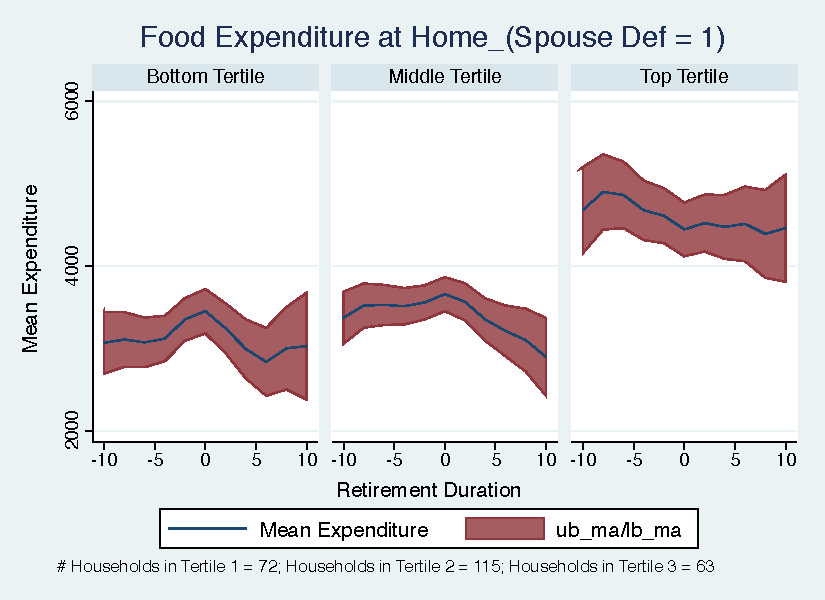
\includegraphics[width=1.0\textwidth]{../ConsumptionPostRetirement_by_SpouseDef_Cats/Smoothed/1/spouse_def_total_foodexp_home_real.pdf}
\end{figure}

% Not sure this is correct
%\begin{table}[h]
%	\centering
%	\begin{tabular}{lccccc} \hline
 & (1) & (2) & (3) & (4) & (5) \\
VARIABLES & test 6 & test 7 & test 8 & test 9 & test 10 \\ \hline
 &  &  &  &  &  \\
2.tertile & 276.9** & -497.2 & 221.3 & 216.5 & 218.4 \\
 & (109.5) & (545.2) & (168.2) & (168.6) & (168.4) \\
3.tertile & 1,025*** & -445.3 & 981.0*** & 982.2*** & 985.8*** \\
 & (112.4) & (847.7) & (176.6) & (177.1) & (176.8) \\
1.retired\#1b.tertile & -153.8 & -98.22 & 32.56 & 31.33 & 35.16 \\
 & (129.0) & (116.1) & (129.6) & (129.7) & (130.4) \\
1.retired\#2.tertile & -66.90 & 61.12 & 137.3 & 137.4 & 137.3 \\
 & (112.7) & (101.8) & (116.8) & (116.9) & (118.1) \\
1.retired\#3.tertile & -202.0* & -228.7** & -88.24 & -90.19 & -87.05 \\
 & (116.8) & (104.5) & (119.7) & (119.7) & (120.2) \\
 &  &  &  &  &  \\
Observations & 4,431 & 4,431 & 4,431 & 4,431 & 4,431 \\
R-squared & 0.033 & 0.002 &  &  &  \\
HH FE & No & Yes & No & No & No \\
Age Dummies & No & No & Yes & Yes & Yes \\
Dummy Children & No & No & No & Yes & Yes \\
Time & No & No & No & No & Yes \\
 Number of pid &  & 559 & 559 & 559 & 559 \\ \hline
\multicolumn{6}{c}{ Standard errors in parentheses} \\
\multicolumn{6}{c}{ *** p$<$0.01, ** p$<$0.05, * p$<$0.1} \\
\end{tabular}

%\end{table}




\clearpage

\subsection{Food Away from Home Expenditure}

\begin{table}[h]
	\centering
	\begin{tabular}{lcccccccccc} \hline
 & (1) & (2) & (3) & (4) & (5) & (6) & (7) & (8) & (9) & (10) \\
VARIABLES & OLS & test 2 & test 3 & test 4 & test 5 & test 6 & test 7 & test 8 & test 9 & test 10 \\ \hline
 &  &  &  &  &  &  &  &  &  &  \\
2.tertile & 358.7*** & 39.44 & 19.37 & 5.623 & 7.865 & 357.8*** & 37.46 & 102.4 & 17.05 & 32.02 \\
 & (22.99) & (54.60) & (54.78) & (54.49) & (54.39) & (91.97) & (394.4) & (393.6) & (393.5) & (392.7) \\
3.tertile & 964.6*** & 68.75 & 43.14 & 49.70 & 61.16 & 699.2*** & 386.2 & 326.1 & 228.8 & 283.3 \\
 & (24.94) & (64.06) & (64.43) & (64.09) & (63.98) & (94.42) & (613.3) & (618.4) & (619.1) & (618.5) \\
1.retired\#1b.tertile & -106.3 & -296.1*** & -221.8** & -221.2** & -218.9** & -412.9*** & -296.1*** & -186.5* & -195.8** & -209.4** \\
 & (79.54) & (83.56) & (91.98) & (91.48) & (91.31) & (108.4) & (83.98) & (98.53) & (98.40) & (98.69) \\
1.retired\#2.tertile & -56.67 & -324.8*** & -265.6*** & -252.7*** & -256.6*** & -362.5*** & -322.2*** & -232.0*** & -228.7** & -258.4*** \\
 & (68.30) & (73.19) & (81.47) & (81.04) & (80.87) & (94.67) & (73.62) & (89.71) & (89.53) & (90.39) \\
1.retired\#3.tertile & 253.9*** & -85.04 & -25.65 & -11.60 & -8.058 & 212.7** & -87.70 & 7.743 & 12.59 & -1.187 \\
 & (70.30) & (75.17) & (84.88) & (84.43) & (84.28) & (98.15) & (75.58) & (92.07) & (91.88) & (92.12) \\
 &  &  &  &  &  &  &  &  &  &  \\
Observations & 49,816 & 49,816 & 49,816 & 49,816 & 49,816 & 4,431 & 4,431 & 4,431 & 4,431 & 4,431 \\
R-squared & 0.038 & 0.001 & 0.006 & 0.017 & 0.021 & 0.047 & 0.009 & 0.038 & 0.043 & 0.049 \\
HH FE & No & Yes & Yes & Yes & Yes & No & Yes & Yes & Yes & Yes \\
Age Dummies & No & No & Yes & Yes & Yes & No & No & Yes & Yes & Yes \\
Dummy Children & No & No & No & Yes & Yes & No & No & No & Yes & Yes \\
Time & No & No & No & No & Yes & No & No & No & No & Yes \\
 Number of pid &  & 12,178 & 12,178 & 12,178 & 12,178 &  & 559 & 559 & 559 & 559 \\ \hline
\multicolumn{11}{c}{ Standard errors in parentheses} \\
\multicolumn{11}{c}{ *** p$<$0.01, ** p$<$0.05, * p$<$0.1} \\
\end{tabular}

\end{table}

\begin{figure}[h]
	\caption{Food Expenditure Away from Home}
	\centering
	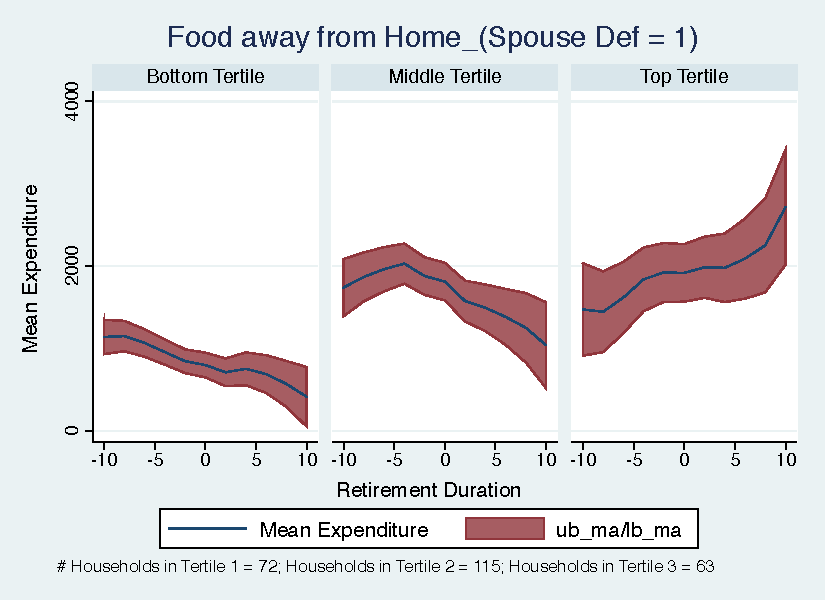
\includegraphics[width=1.0\textwidth]{../ConsumptionPostRetirement_by_SpouseDef_Cats/Smoothed/1/spouse_def_total_foodexp_away_real.pdf}
\end{figure}
\clearpage

\subsection{Education Expenditure}
\begin{table}[h]
	\centering
	\begin{tabular}{lccccc} \hline
 & (1) & (2) & (3) & (4) & (5) \\
VARIABLES & OLS & test 2 & test 3 & test 4 & test 5 \\ \hline
 &  &  &  &  &  \\
1.retired & -560.5*** & -849.8*** & -179.7 & -188.1 & -186.0 \\
 & (94.33) & (119.0) & (130.2) & (129.5) & (129.5) \\
 &  &  &  &  &  \\
Observations & 69,862 & 69,862 & 69,862 & 69,862 & 69,862 \\
R-squared & 0.001 & 0.001 & 0.016 & 0.026 & 0.026 \\
HH FE & No & Yes & Yes & Yes & Yes \\
Age Dummies & No & No & Yes & Yes & Yes \\
Dummy Children & No & No & No & Yes & Yes \\
Time & No & No & No & No & Yes \\
 Number of pid &  & 18,085 & 18,085 & 18,085 & 18,085 \\ \hline
\multicolumn{6}{c}{ Standard errors in parentheses} \\
\multicolumn{6}{c}{ *** p$<$0.01, ** p$<$0.05, * p$<$0.1} \\
\end{tabular}

\end{table}

\begin{figure}[h]
	\caption{Expenditure on Education}
	\centering
	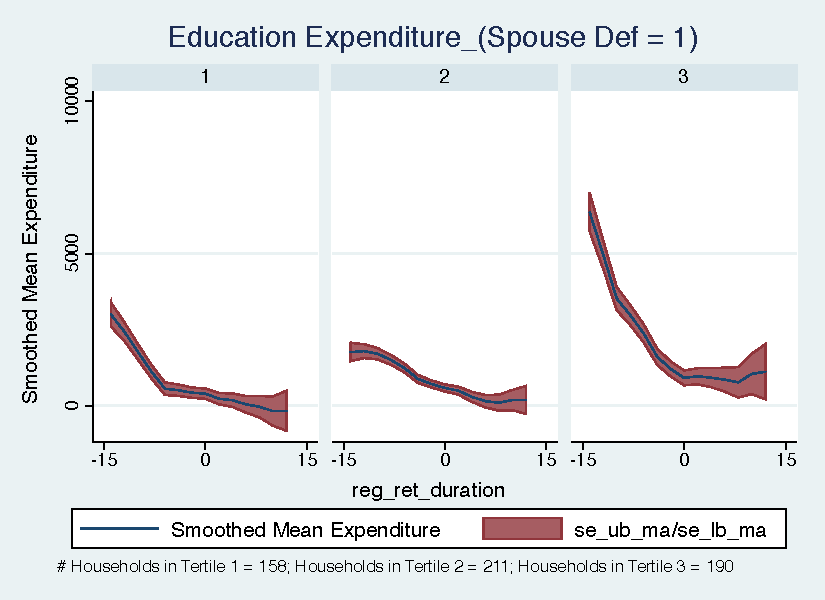
\includegraphics[width=1.0\textwidth]{../ConsumptionPostRetirement_by_SpouseDef_Cats/Smoothed/1/spouse_def_total_education_real.pdf}
\end{figure}
\clearpage

\subsection{Health Expenditure}
(Previously labeled recreation expenditure. But the tex file says health expenditure.)

\begin{table}[h]
	\centering
	\begin{tabular}{lccccc} \hline
 & (1) & (2) & (3) & (4) & (5) \\
VARIABLES & OLS & test 2 & test 3 & test 4 & test 5 \\ \hline
 &  &  &  &  &  \\
1.retired & 1,372*** & 1,173*** & 506.5*** & 505.0*** & 509.9*** \\
 & (93.19) & (119.2) & (129.3) & (129.3) & (129.2) \\
 &  &  &  &  &  \\
Observations & 69,862 & 69,862 & 69,862 & 69,862 & 69,862 \\
R-squared & 0.003 & 0.002 & 0.033 & 0.033 & 0.034 \\
HH FE & No & Yes & Yes & Yes & Yes \\
Age Dummies & No & No & Yes & Yes & Yes \\
Dummy Children & No & No & No & Yes & Yes \\
Time & No & No & No & No & Yes \\
 Number of pid &  & 18,085 & 18,085 & 18,085 & 18,085 \\ \hline
\multicolumn{6}{c}{ Standard errors in parentheses} \\
\multicolumn{6}{c}{ *** p$<$0.01, ** p$<$0.05, * p$<$0.1} \\
\end{tabular}

\end{table}

\begin{figure}[h]
	\caption{Expenditure on Health}
	\centering
	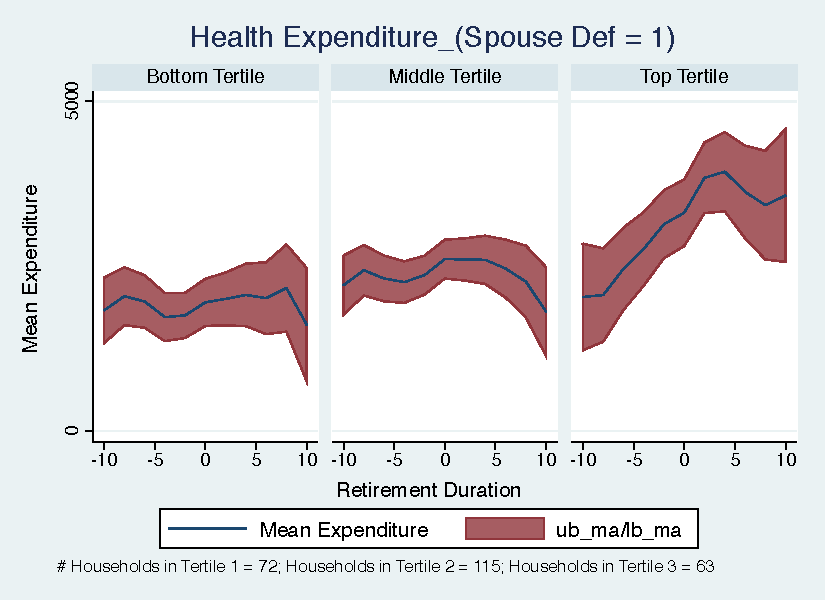
\includegraphics[width=1.0\textwidth]{../ConsumptionPostRetirement_by_SpouseDef_Cats/Smoothed/1/spouse_def_total_healthexpense_real.pdf}
\end{figure}
\clearpage

\subsection{Housing Expenditure}
\begin{table}[h]
	\centering
	\begin{tabular}{lccccc} \hline
 & (1) & (2) & (3) & (4) & (5) \\
VARIABLES & test 6 & test 7 & test 8 & test 9 & test 10 \\ \hline
 &  &  &  &  &  \\
2.tertile & 1,969*** & -222.7 & 404.9 & 532.5 & 608.7 \\
 & (607.5) & (969.1) & (761.7) & (757.2) & (746.2) \\
3.tertile & 5,128*** & -1,074 & 2,458*** & 2,507*** & 2,790*** \\
 & (567.0) & (1,638) & (918.4) & (910.0) & (903.5) \\
1.retired\#1b.tertile & 726.0 & -27.41 & -1,347*** & -1,337*** & -719.1 \\
 & (781.5) & (439.6) & (475.2) & (473.6) & (470.1) \\
1.retired\#2.tertile & -1,633*** & 138.0 & -828.5** & -867.5** & -514.5 \\
 & (617.9) & (343.2) & (393.9) & (392.7) & (386.7) \\
1.retired\#3.tertile & 877.2* & 561.0** & -143.6 & -125.1 & 122.3 \\
 & (498.6) & (272.5) & (344.6) & (343.4) & (337.4) \\
 &  &  &  &  &  \\
Observations & 4,431 & 4,431 & 4,431 & 4,431 & 4,431 \\
R-squared & 0.043 & 0.001 &  &  &  \\
HH FE & No & Yes & No & No & No \\
Age Dummies & No & No & Yes & Yes & Yes \\
Dummy Children & No & No & No & Yes & Yes \\
Time & No & No & No & No & Yes \\
 Number of pid &  & 559 & 559 & 559 & 559 \\ \hline
\multicolumn{6}{c}{ Standard errors in parentheses} \\
\multicolumn{6}{c}{ *** p$<$0.01, ** p$<$0.05, * p$<$0.1} \\
\end{tabular}

\end{table}

\begin{figure}[h]
	\caption{Expenditure on Housing}
	\centering
	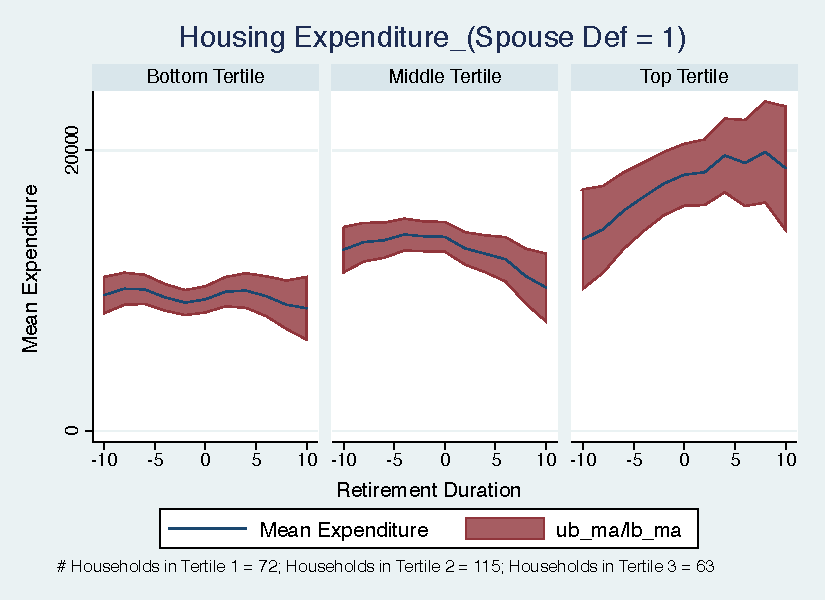
\includegraphics[width=1.0\textwidth]{../ConsumptionPostRetirement_by_SpouseDef_Cats/Smoothed/1/spouse_def_total_housing_real.pdf}
\end{figure}
\clearpage

\subsection{Nondurable Transportation Expenditure}
\begin{table}[h]
	\centering
	\begin{tabular}{lcccccccccc} \hline
 & (1) & (2) & (3) & (4) & (5) & (6) & (7) & (8) & (9) & (10) \\
VARIABLES & OLS & test 2 & test 3 & test 4 & test 5 & test 6 & test 7 & test 8 & test 9 & test 10 \\ \hline
 &  &  &  &  &  &  &  &  &  &  \\
2.tertile & 870.2*** & 124.2 & 4.195 & -28.04 & -30.52 & 406.1 & 740.1 & 755.3 & 542.2 & 734.8 \\
 & (57.92) & (175.0) & (173.2) & (172.7) & (172.1) & (278.1) & (1,686) & (1,514) & (1,516) & (1,510) \\
3.tertile & 1,426*** & -39.90 & -206.7 & -197.0 & -137.9 & 1,215*** & 481.6 & -435.7 & -479.6 & 159.0 \\
 & (62.84) & (205.3) & (203.7) & (203.2) & (202.5) & (285.5) & (2,622) & (2,379) & (2,384) & (2,379) \\
1.retired\#1b.tertile & -143.3 & -619.3** & -252.7 & -246.6 & -325.5 & -941.8*** & -614.1* & -463.0 & -465.2 & -336.6 \\
 & (200.4) & (267.8) & (290.8) & (290.0) & (289.0) & (327.9) & (359.0) & (379.1) & (379.0) & (379.6) \\
1.retired\#2.tertile & -516.9*** & -605.6*** & -271.2 & -241.7 & -297.4 & -851.2*** & -609.9* & -522.5 & -506.3 & -341.3 \\
 & (172.1) & (234.5) & (257.6) & (256.9) & (256.0) & (286.3) & (314.7) & (345.1) & (344.8) & (347.7) \\
1.retired\#3.tertile & 73.55 & -926.1*** & -681.6** & -651.7** & -732.7*** & -513.3* & -925.3*** & -918.8*** & -907.9** & -777.9** \\
 & (177.1) & (240.9) & (268.3) & (267.7) & (266.7) & (296.8) & (323.1) & (354.2) & (353.9) & (354.3) \\
 &  &  &  &  &  &  &  &  &  &  \\
Observations & 49,816 & 49,816 & 49,816 & 49,816 & 49,816 & 4,431 & 4,431 & 4,431 & 4,431 & 4,431 \\
R-squared & 0.011 & 0.001 & 0.033 & 0.038 & 0.045 & 0.014 & 0.004 & 0.217 & 0.219 & 0.227 \\
HH FE & No & Yes & Yes & Yes & Yes & No & Yes & Yes & Yes & Yes \\
Age Dummies & No & No & Yes & Yes & Yes & No & No & Yes & Yes & Yes \\
Dummy Children & No & No & No & Yes & Yes & No & No & No & Yes & Yes \\
Time & No & No & No & No & Yes & No & No & No & No & Yes \\
 Number of pid &  & 12,178 & 12,178 & 12,178 & 12,178 &  & 559 & 559 & 559 & 559 \\ \hline
\multicolumn{11}{c}{ Standard errors in parentheses} \\
\multicolumn{11}{c}{ *** p$<$0.01, ** p$<$0.05, * p$<$0.1} \\
\end{tabular}

\end{table}

\begin{figure}[h]
	\caption{Expenditure on Nondurable Transport}
	\centering
	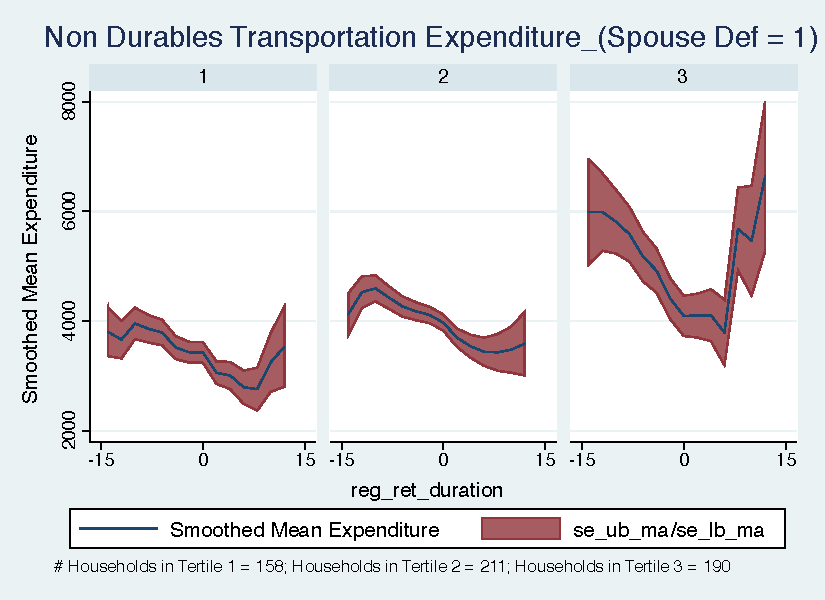
\includegraphics[width=1.0\textwidth]{../ConsumptionPostRetirement_by_SpouseDef_Cats/Smoothed/1/spouse_def_total_transport_real.pdf}
\end{figure}
\clearpage

\subsection{Recreation Expenditure}
\begin{table}[h]
	\centering
	\begin{tabular}{lccccc} \hline
 & (1) & (2) & (3) & (4) & (5) \\
VARIABLES & test 6 & test 7 & test 8 & test 9 & test 10 \\ \hline
 &  &  &  &  &  \\
2.tertile & 1,625*** & 1,106 & 1,651** & 1,658** & 1,714*** \\
 & (531.0) & (1,295) & (652.3) & (650.4) & (651.5) \\
3.tertile & 2,187*** & 5,463** & 2,524*** & 2,498*** & 2,604*** \\
 & (495.8) & (2,135) & (641.6) & (639.4) & (643.9) \\
1.retired\#1b.tertile & 441.3 & 250.8 & 967.6* & 941.5 & 812.8 \\
 & (573.5) & (584.2) & (587.4) & (587.5) & (601.8) \\
1.retired\#2.tertile & -1,521*** & -1,329*** & -791.2 & -816.6* & -950.5* \\
 & (468.7) & (476.4) & (490.8) & (491.2) & (504.4) \\
1.retired\#3.tertile & -147.7 & -142.7 & 291.5 & 293.2 & 132.7 \\
 & (385.4) & (387.2) & (412.4) & (412.3) & (430.8) \\
 &  &  &  &  &  \\
Observations & 2,984 & 2,984 & 2,984 & 2,984 & 2,984 \\
R-squared & 0.016 & 0.006 &  &  &  \\
HH FE & No & Yes & No & No & No \\
Age Dummies & No & No & Yes & Yes & Yes \\
Dummy Children & No & No & No & Yes & Yes \\
Time & No & No & No & No & Yes \\
 Number of pid &  & 559 & 559 & 559 & 559 \\ \hline
\multicolumn{6}{c}{ Standard errors in parentheses} \\
\multicolumn{6}{c}{ *** p$<$0.01, ** p$<$0.05, * p$<$0.1} \\
\end{tabular}

\end{table}

\begin{figure}[h]
	\caption{Expenditure on total recreation (post 2005)}
	\centering
	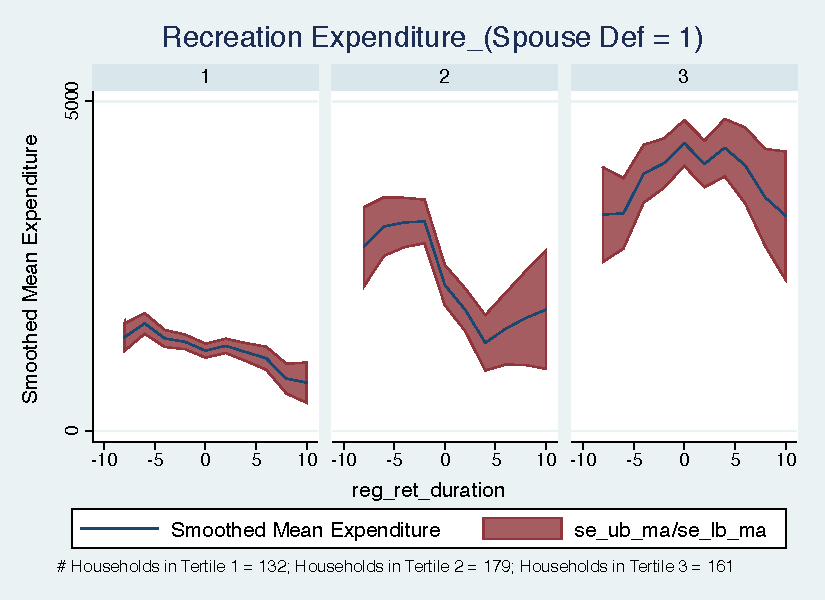
\includegraphics[width=1.0\textwidth]{../ConsumptionPostRetirement_by_SpouseDef_Cats/Smoothed/1/spouse_def_total_recreation_2005_real.pdf}
\end{figure}

\clearpage

\subsection{Clothing Expenditure}
\begin{table}[h]
	\centering
	\begin{tabular}{lccccc} \hline
 & (1) & (2) & (3) & (4) & (5) \\
VARIABLES & test 6 & test 7 & test 8 & test 9 & test 10 \\ \hline
 &  &  &  &  &  \\
2.tertile & 32.19 & 90.67 & 132.6 & 133.6 & 99.50 \\
 & (124.2) & (316.4) & (151.7) & (151.8) & (151.9) \\
3.tertile & 231.4** & 179.1 & 417.4*** & 413.6*** & 352.1** \\
 & (116.0) & (521.8) & (148.0) & (148.1) & (149.0) \\
1.retired\#1b.tertile & -507.0*** & -428.2*** & -185.3 & -188.3 & -111.4 \\
 & (134.1) & (142.8) & (141.5) & (141.6) & (144.7) \\
1.retired\#2.tertile & -565.9*** & -460.9*** & -287.2** & -291.8** & -215.0* \\
 & (109.6) & (116.4) & (118.2) & (118.4) & (121.3) \\
1.retired\#3.tertile & -315.1*** & -383.9*** & -147.6 & -146.0 & -47.34 \\
 & (90.13) & (94.63) & (99.08) & (99.12) & (103.4) \\
 &  &  &  &  &  \\
Observations & 2,984 & 2,984 & 2,984 & 2,984 & 2,984 \\
R-squared & 0.026 & 0.017 &  &  &  \\
HH FE & No & Yes & No & No & No \\
Age Dummies & No & No & Yes & Yes & Yes \\
Dummy Children & No & No & No & Yes & Yes \\
Time & No & No & No & No & Yes \\
 Number of pid &  & 559 & 559 & 559 & 559 \\ \hline
\multicolumn{6}{c}{ Standard errors in parentheses} \\
\multicolumn{6}{c}{ *** p$<$0.01, ** p$<$0.05, * p$<$0.1} \\
\end{tabular}

\end{table}

\begin{figure}[h]
	\caption{Expenditure on total clothing (post 2005)}
	\centering
	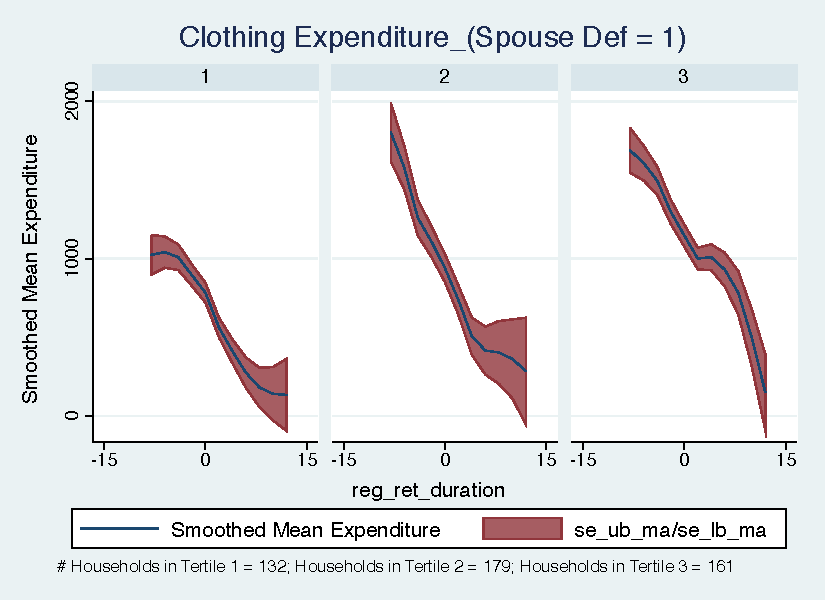
\includegraphics[width=1.0\textwidth]{../ConsumptionPostRetirement_by_SpouseDef_Cats/Smoothed/1/spouse_def_total_clothing_2005_real.pdf}
\end{figure}

\clearpage




\end{document}
              